\section{Strong-Anchor and Representation Follow-Up}
The follow-up specification is a timestamped local plan, not public preregistration. All added comparisons on previously evaluated families are exploratory. The original evidence files are hash checked and the original numerical/full predictions are re-fitted to absolute tolerance $10^{-12}$ before each numerical analysis. Focal comparisons do not replace the historical locally locked decision rules.

\subsection{Anchor ladder and a VLM-free estimator}
The Laplace control fits the joint physical/nuisance Gaussian MAP under original bounds and observation precision. A Gauss--Newton local Gaussian approximation is marginalized over nuisance by a Schur complement. Its physical mean equals the joint mode; it does not integrate a non-Gaussian posterior or profile dispersion. All 1,440 distinct fits converge, with no nuisance-bound contact or rank deficiency. The VLM-free profiled-MAP control uses a development population prior and observation-derived nuisance starts, with no appearance features or original-prior initialization. It uses the same cached calibrated RGB tracking measurements, and is not a matched residual-head ablation. One failed fit is retained.

\begin{table}[htbp]\centering\small
\caption{Added Classical Controls}\label{tab:fu_anchors}
\begin{tabular}{lrr}\toprule
Method & MAE (mm) & Convergence\\\midrule
Laplace marginal & 1.918031 & 100.00\%\\
VLM-free population MAP & 1.866472 & 99.93\%\\
\bottomrule\end{tabular}
\end{table}
\subsection{Matched dimensionality and missing numerical cell}
The 87-dimensional view concatenates nine dynamic channels across eight frames (72 values) with one copy of 15 setup channels. Numerical penalties $\{0.1,1,10\}$ use the original six family folds; 0.1 minimizes the numerical-only development loss. The four visual representations are compared above that same numerical fit. Their penalties $\{1,10,100\}$ use the same folds; neither evaluation targets nor errors select any setting. Development scores remain selection scores. The PCA fitting sets exclude validation families, and all final fits use development families only.

\begin{table}[htbp]\centering\small
\caption{Representation Ladder with Development-Selected Penalties}\label{tab:fu_repr}
\begin{tabular}{lrrrr}\toprule
Arm & Numeric $\lambda$ & Visual $\lambda$ & Dev. mm & Eval. mm\\\midrule
numeric192 & 1 & 0 & 1.37193 & 1.46877\\
full192 & 1 & 10 & 1.35223 & 1.45312\\
numeric87 & 0.1 & 0 & 1.36567 & 1.44213\\
qwen87 & 0.1 & 10.0 & 1.34792 & 1.42632\\
flow87 & 0.1 & 1.0 & 1.35202 & 1.41695\\
pixels87 & 0.1 & 100.0 & 1.36595 & 1.43405\\
vjepa87 & 0.1 & 100.0 & 1.37007 & 1.44407\\
\bottomrule\end{tabular}
\end{table}
The classical extractor uses only the same eight hash-checked grayscale RGB frames and the original first-frame object cue. Up to 64 ROI corners are propagated with pyramidal Lucas--Kanade (21-pixel window, three pyramid levels, 30 iterations, 0.01 tolerance). Median point displacement defines a centroid trajectory. The 48 features are seven horizontal and seven vertical displacements, six horizontal and six vertical second differences, seven horizontal direction cosines, seven point-spread ratios, and eight aggregate flow/failure/appearance-change statistics. Image dimensions normalize displacement. Zero successful tracks yields zero displacement and a failure count; no episode is removed. The evaluation set has 1,189 failed transitions of 7,560. Raw pixels are eight 16-by-16 grayscale frames followed by training-fold PCA-48. These controls are specified implementations, not optimized non-neural performance bounds. DINO, ResNet and text-generation arms are not claimed as completed. Upstream decoder supervision is not matched across encoder families.

\begin{figure}[htbp]\centering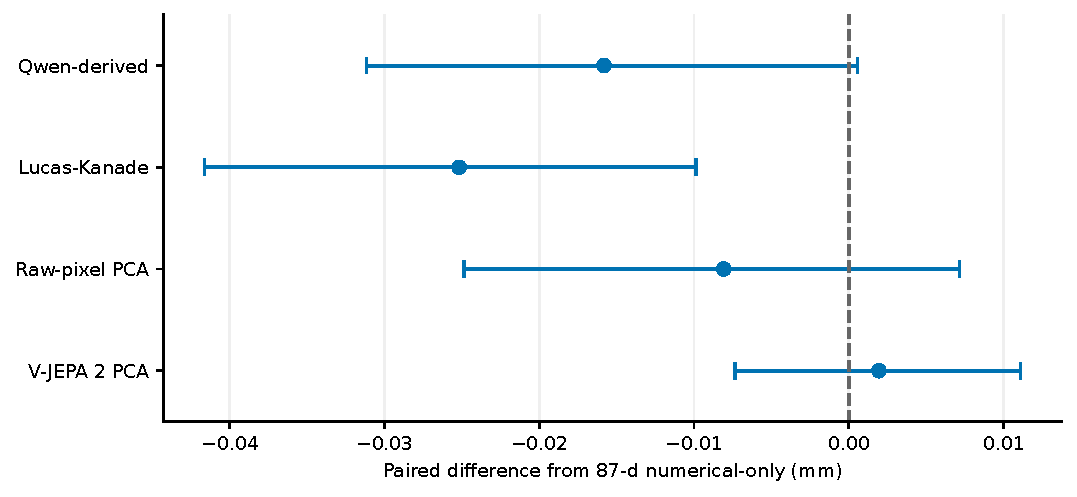
\includegraphics[width=.9\textwidth]{figures/representation_ladder.pdf}
\caption{Exploratory paired 95\% mean-error intervals relative to the strengthened numerical comparator. Interval overlap or inclusion of zero is not evidence of equivalence.}\end{figure}
\subsection{Multiplicity and effect interpretation}
Three focal comparisons use 20,000 paired family draws and two-sided sign-flip mean tests, with Holm adjustment within those three. A broader sensitivity applies Holm to 59 unique available family-action comparisons, removing duplicate prediction vectors and retaining unsuccessful baselines. The full list is in \path{replayed/followup/global_action_holm.csv}. This correction does not undo adaptive study history, selected penalties or repeated cohort use. Public episode bootstrap contrasts, correlation diagnostics, and covariance summary curves concern different estimands and remain explicitly descriptive; they are not new confirmatory discoveries. No statistical equivalence margin was specified.

\begin{table}[htbp]\centering\small
\caption{Focal Exploratory Contrasts (72 Families)}\label{tab:fu_focal}
\begin{tabular}{lrrr}\toprule
Contrast & $\Delta$ mm & 95\% interval & Holm $p$\\\midrule
full192 minus profiled MAP & -0.37003 & [-0.56199, -0.18024] & 0.00150\\
qwen87 minus flow87 & +0.00936 & [-0.01054, +0.03061] & 0.37728\\
qwen87 minus numeric87 & -0.01582 & [-0.03114, +0.00057] & 0.10139\\
\bottomrule\end{tabular}
\end{table}
\subsection{Capacity and latency}
Stored coefficient counts include intercepts and both setup branches: 1,544 numerical plus 392 visual coefficients for the original full model, and 704 plus 392 for the deduplicated full model. Excluding the generalized-bounce fallback branch yields 959 active coefficients for the deduplicated full model. The 328,356-parameter upstream observation decoder is separately trained and is excluded from these residual counts. PCA storage and encoder weights are not residual coefficients. The original component sums (129.1 and 362.5 ms) use staged model-resident GPU measurements; the 68.4-ms first-image prior is shared. Classical feature extraction is measured separately and cannot be added to those GPU totals to claim end-to-end acceleration. No full-path timing is imputed for unmeasured arms.
\begin{figure}[htbp]\centering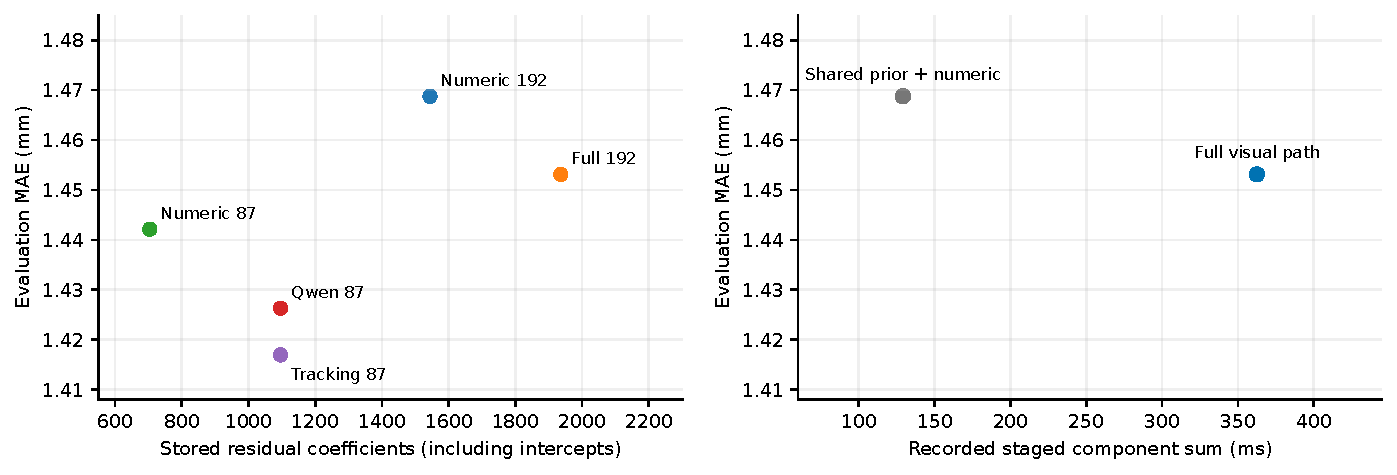
\includegraphics[width=\textwidth]{figures/capacity_latency.pdf}
\caption{Residual capacity versus error, and the two existing full-path component measurements. Neither panel isolates pretraining; the right panel omits unmeasured timings.}\end{figure}
\subsection{Feature-unit correction in real video}
The original 33-video inference is reconstructed with exactly matching raw scores. Both projected pixel-correction channels are divided by a tracking-noise proxy: 1.4826 times quadratic-detrended median absolute deviation, floored at one resized-image pixel. The resulting scale spans 1.000--1.077 pixels, so the intervention is small. Pooled states are unchanged. The operation matches dimensional form, not camera geometry or domain distributions. The 152-frame bridge uses deceleration/initial-speed and a camera indicator; scaling both numerator and denominator leaves the ratio invariant. Its scalar proxy is invariant for the same reason. The corrected short score is still not a friction estimate.

\begin{table}[htbp]\centering\small
\caption{Original and Unit-Normalized Real-Video Correlations}\label{tab:fu_real}
\begin{tabular}{lrrr}\toprule
Arm & Stage & Family $\rho$ & Bootstrap 95\%\\\midrule
combined & original & -0.700 & [-0.972, -0.121]\\
combined & noise\_normalized & -0.700 & [-0.972, -0.121]\\
pooled & original & 0.027 & [-0.571, 0.735]\\
pooled & noise\_normalized & 0.027 & [-0.571, 0.735]\\
position & original & -0.455 & [-0.944, 0.306]\\
position & noise\_normalized & -0.455 & [-0.944, 0.306]\\
kinematic\_short & original & 0.127 & [-0.713, 0.793]\\
kinematic\_short & noise\_normalized & 0.127 & [-0.713, 0.793]\\
bridge\_152frame & original & 0.355 & [-0.411, 0.869]\\
bridge\_152frame & normalized & 0.355 & [-0.411, 0.869]\\
scalar\_152frame & original & 0.427 & [-0.310, 0.906]\\
scalar\_152frame & normalized & 0.427 & [-0.310, 0.906]\\
\bottomrule\end{tabular}
\end{table}
\subsection{Independent-family calibration}
Forty new geometry families (600 RGB episodes) are generated using separate geometry and physics seed streams. Physical shape hashes are checked against prior geometry manifests. Generation-side targets are stored separately. The predictor is denied access to the target directory and records a hash/timestamp seal before calibration labels are opened. The original appearance prior, observation decoder and residual checkpoint are frozen. No model is fitted to calibration labels. Beta is selected by development CRPS, with no evaluation-coverage tuning.

For each family a fixed seed chooses one of its 30 episode/setup combinations uniformly, independently of residual values. The 37th order statistic of 40 normalized Mahalanobis scores defines the representative-family conformal scale. Its exchangeability target is a randomly sampled episode/setup of a new family. A separate 37th order statistic of within-family maxima targets simultaneous coverage of all such observations. Marginal and simultaneous-family coverage are different events; neither implies protocol-conditional nominal coverage. Evaluation on the previously inspected 72 families is descriptive and was not used to choose the quantile.
The selected $\beta$ is 0; representative-family $\hat q=0.44212$ and maximum-family $\hat q=7.91249$.

\begin{table}[htbp]\centering\small
\caption{Independent-Calibration Coverage on the Existing Evaluation Set}\label{tab:fu_cal}
\begin{tabular}{lrrr}\toprule
Region & Protocol & Coverage & Family-all\\\midrule
Unscaled & all & 96.81\% & 68.06\%\\
Unscaled & multiple forces & 91.94\% & 73.61\%\\
Unscaled & unforced slide & 100.00\% & 100.00\%\\
Unscaled & bounce & 98.47\% & 90.28\%\\
Representative & all & 81.94\% & 13.89\%\\
Representative & multiple forces & 67.22\% & 34.72\%\\
Representative & unforced slide & 91.94\% & 77.78\%\\
Representative & bounce & 86.67\% & 40.28\%\\
Family maximum & all & 99.86\% & 95.83\%\\
Family maximum & multiple forces & 100.00\% & 100.00\%\\
Family maximum & unforced slide & 100.00\% & 100.00\%\\
Family maximum & bounce & 99.58\% & 95.83\%\\
\bottomrule\end{tabular}
\end{table}
The public 53-episode empirical calibration is preserved and is not promoted to split conformal. A new independent public material-calibration partition is not implemented here. The new synthetic calibration assesses only its stated family sampling regime and fails the specified episode-coverage target; evaluation outcomes are not used to retune it.
\subsection{Scope of implemented extensions}
The protocol mask remains an assumption-driven restriction supported by elementary dynamics, not a newly proved Fisher-information rule. A final-solution automatic-mask policy, matched-supervision encoder 2-by-2 experiment, external text/simulator method ports, and three-axis asset/physics/sensor stress study are not included. The new independent geometries are calibration samples, not a model-misspecification or multi-object transfer benchmark. No equivalence or language-pretraining conclusion relies on missing cells. The original direct-regression and failed-transfer results remain in the preceding exploratory sections.
